\documentclass{article}     % libraries / packages just like modules in python
                            % Starts an article
\usepackage{amsmath}        %AMS mathematical facilities for LaTeX
\usepackage[utf8]{inputenc} % Or like Just like adding HEader files in C++
%*******************
\usepackage{geometry}
\usepackage{pdfpages} 
\usepackage[english]{babel} 
\addto{\captionenglish}{
  \renewcommand{\bibname}{References}
}     % package used to define the layout of the document
 	\geometry
 		{
 			a4paper,        % To define the aspect ratio of the doc
 			%total={170mm,257mm},
 			left=25mm,
 			top=25mm,
 			right=20mm,
 			bottom=20mm,
 		}
\title{\LaTeX{}}             % Main heading of the document
\author{Author: Abhijith S} % For specifying Author of the document
\date{Date: October 2021}   % For specifying Date of the document
%*******************
%the section in between the stars makes 
%up the title part 

%the code till now is called preample

\begin{document} %Beginning of document just like <html> tag

\centering
\tableofcontents %This command used for index.
\listoffigures
\maketitle
  \LaTeX{} is a document preparation system for
  the \TeX{} typesetting program. It offers
  programmable desktop publishing features and
  extensive facilities for automating most
  aspects of typesetting and desktop publishing,
  including numbering and  cross-referencing,
  tables and figures, page layout,
  bibliographies, and much more. \LaTeX{} was
  originally written in 1984 by Leslie Lamport
  and has become the  dominant method for using
  \TeX; few people write in plain \TeX{} anymore.
  The current version is \LaTeXe.

  % This is a comment, not shown in final output.
  % The following shows typesetting  power of LaTeX:
  \begin{align}
    E_0 &= mc^2 \\
    E &= \frac{mc^2}{\sqrt{1-\frac{v^2}{c^2}}}
  \end{align} 


%************************************************
%title of the document / main heading
% This is what the code that makes the title 
%appear at the top of the document

\section{Introduction}
%Sub section of the document numbered the
%first beginning from one numerical
% "Introduction" is only a heading 

This text would appear just from the left side below the introduction
\newline
Let's Begin with a formula  $e^{i\pi}+1 = 0$. 
\newline
But we can also do 
$$e =  \lim_{n\to\infty}\left(1+ \frac{1}{n}\right)^n = \lim_{n\to\infty}\frac{n}{\sqrt[n]{n!}}$$
%we can code of formulas in between two dollar
%signs
we can do another: $$e = \sum_{n=0}^{\infty}\frac{1}{n!}$$

\section{Just another Section}
     Just some text under this section 
     \subsection{A subsection}
Whatever code put in here would be shown as same as they are written:

\begin{verbatim}
  //Whatever code put in here would be shown as same as they are written
    class _WeatherPageState extends State<WeatherPage> {
  @override
  void initState() {
    getweather();
    super.initState();
  }

  WeatherFactory wf = new WeatherFactory("9e8638e0e66018f75db6fc0ed9512f3b");
  late Weather mylocation;
  bool loading = true;
  getweather() async {
      await Geolocator.requestPermission();
    print('gotlocation');
\end{verbatim}

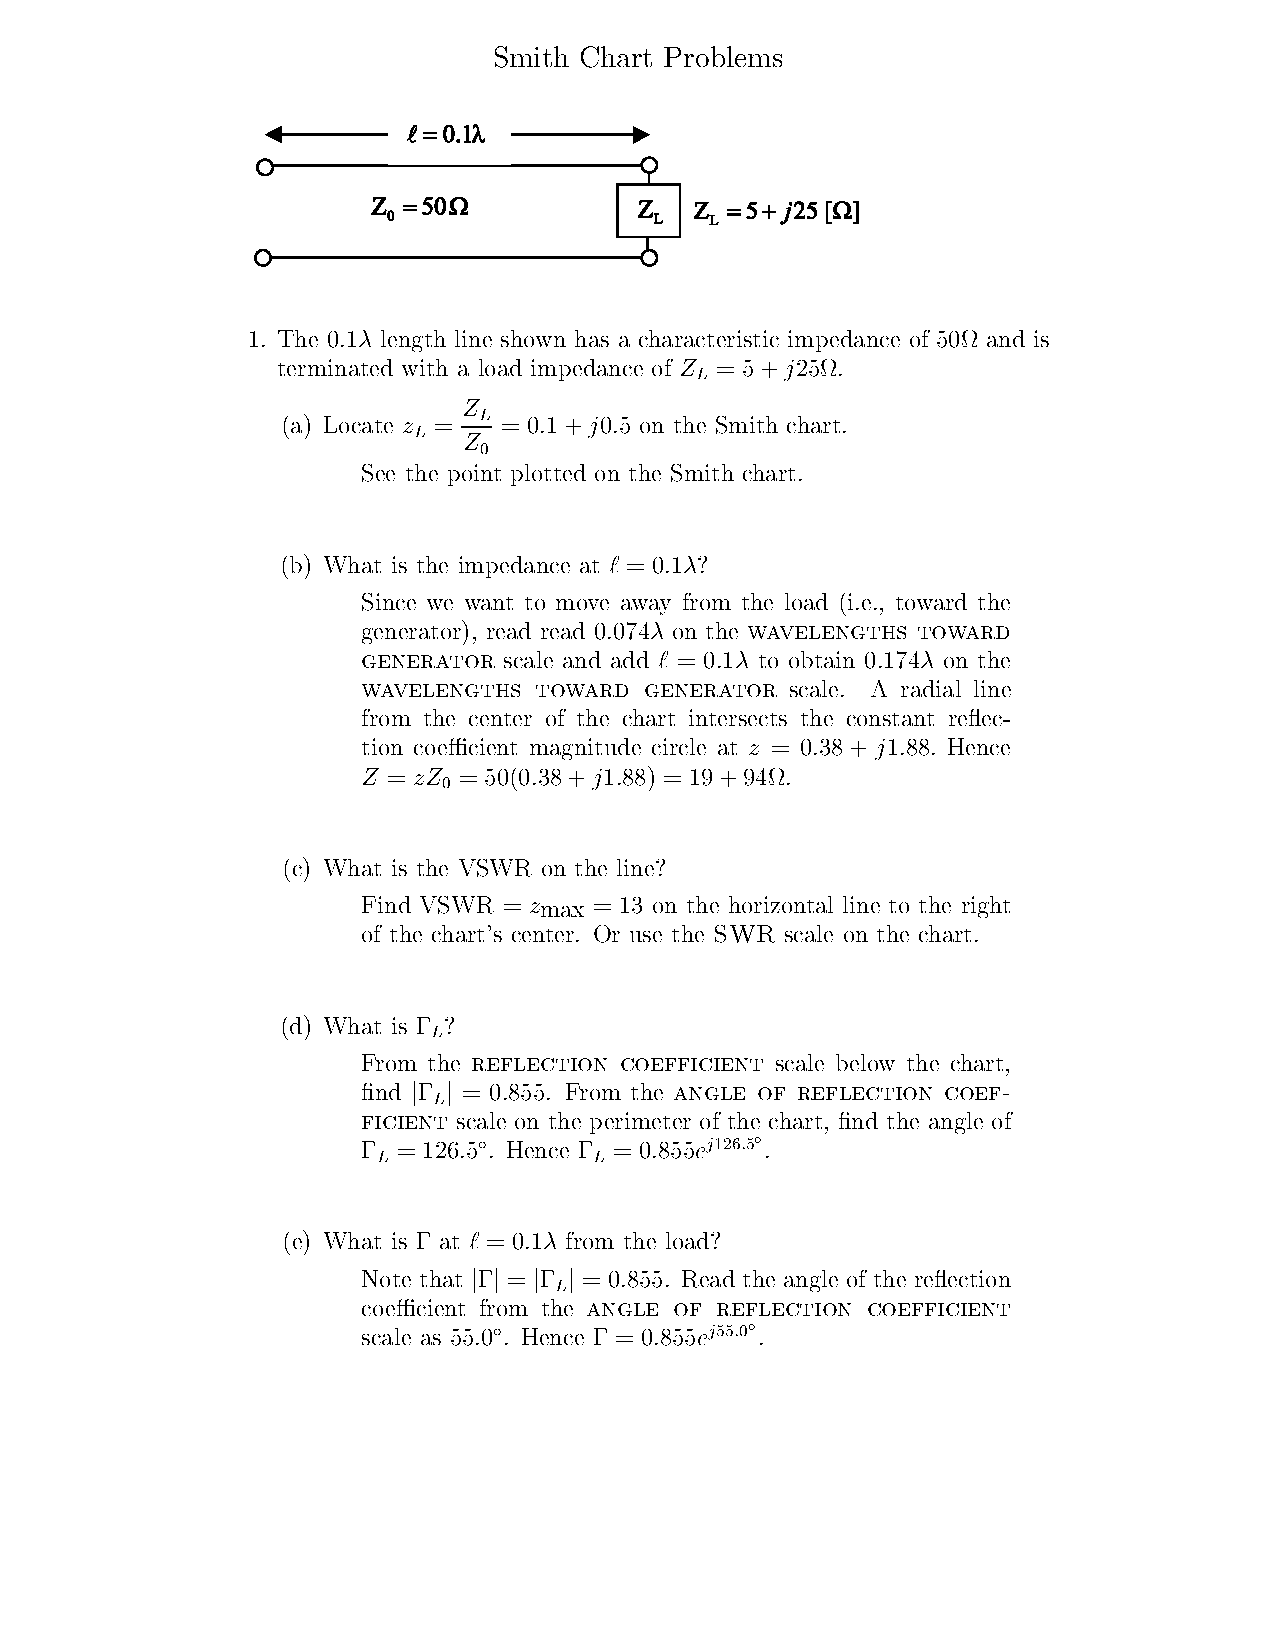
\includepdf[scale=0.5, page={2,4}, offset=100 190]{smithcht}
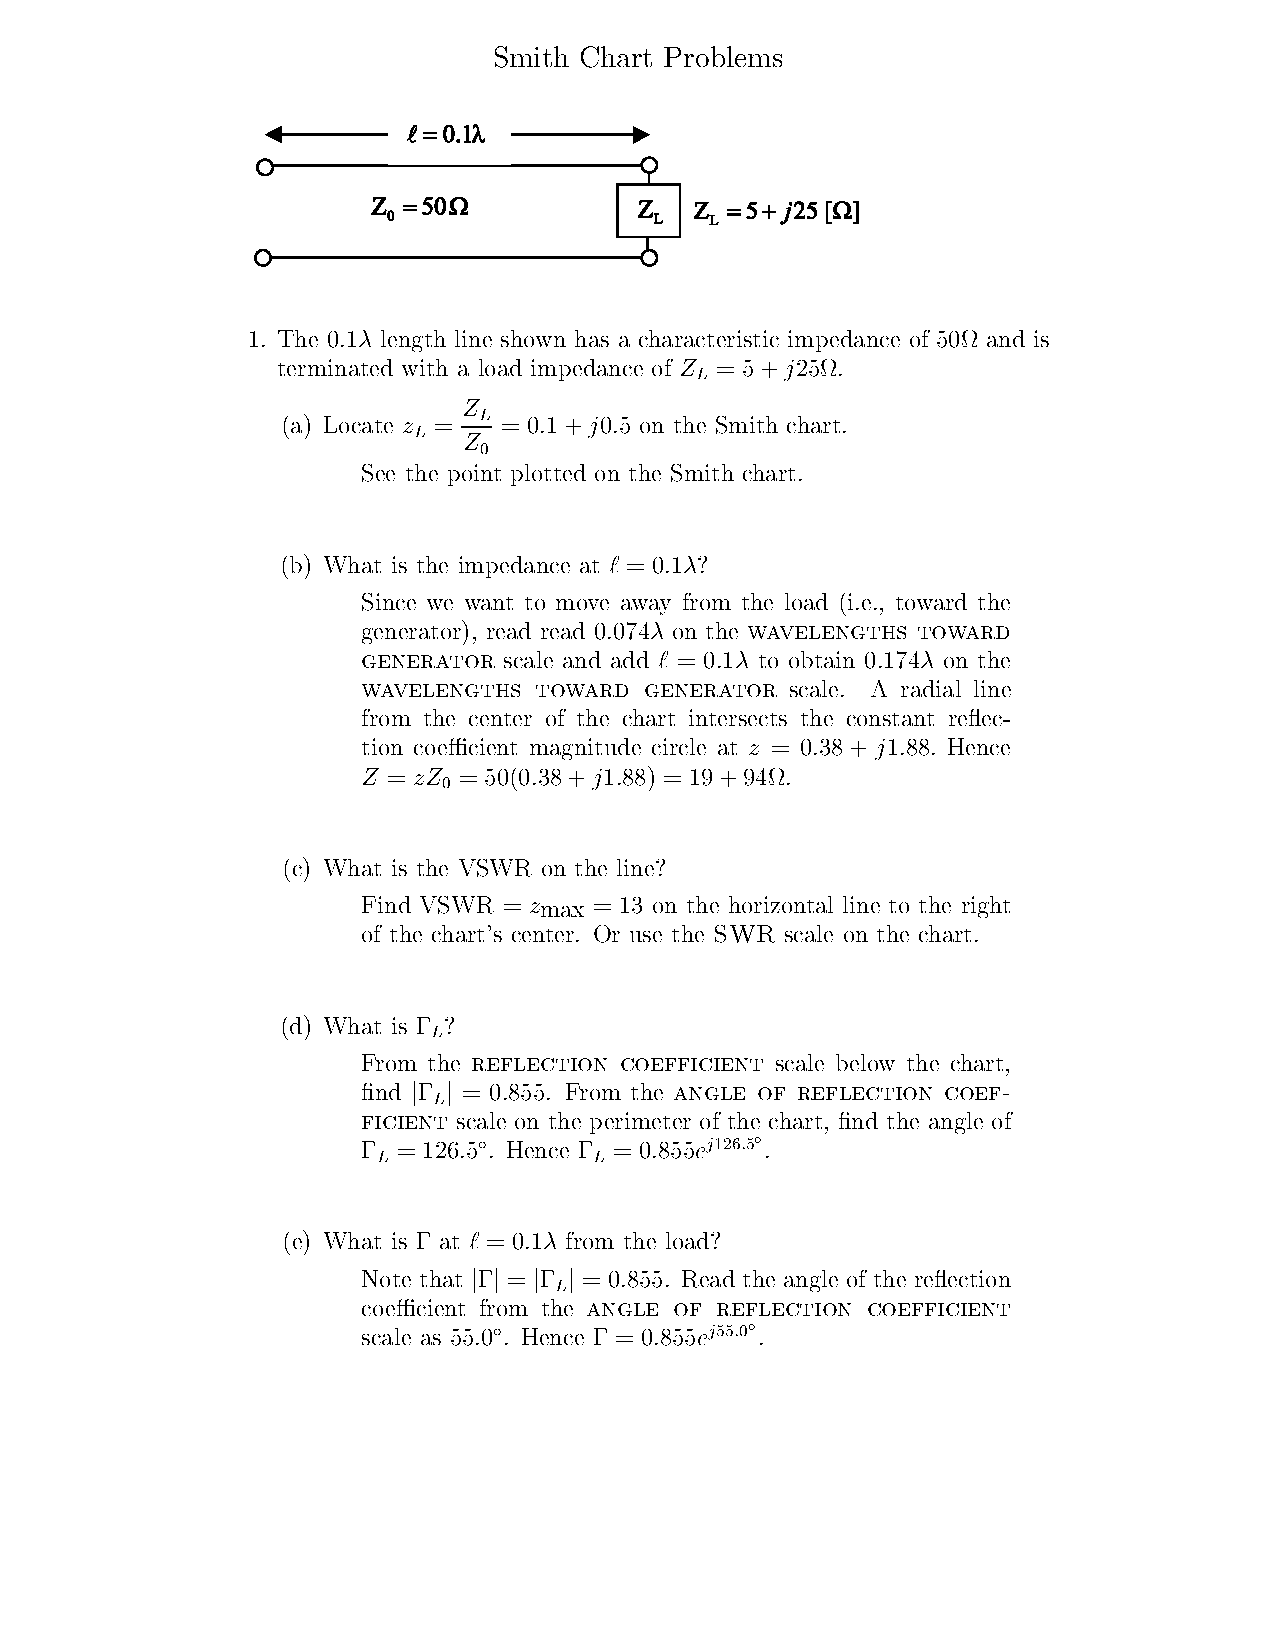
\includepdf[page={4}]{smithcht}
\subsection{next subsection}
Text under subsection:  
putting some lorem ipsum to make it look like there is some text under this. 
Lorem Ipsum is simply dummy text of the printing and typesetting industry. 
Lorem Ipsum has been the industry's standard dummy text ever since the 1500s, 
when an unknown printer took a galley of type and scrambled it to make a type 
specimen book. It has survived not only five centuries, but also the leap into 
electronic typesetting, remaining essentially unchanged. It was popularised in 
the 1960s with the release of Letraset sheets containing Lorem Ipsum passages, 
and more recently with desktop publishing software like Aldus PageMaker 
including versions of Lorem Ipsum.
\subsubsection{a sub sub section :)}

It is a long established fact that a reader will be distracted by the readable 
content of a page when looking at its layout. The point of using Lorem Ipsum is
 that it has a more-or-less normal distribution of letters, as opposed to using 
 'Content here, content here', making it look like readable English. 
 Many desktop publishing packages and web page editors now use Lorem Ipsum as 
 their default model text, and a search for 'lorem ipsum' will uncover many 
 web sites still in their infancy. Various versions have evolved over the years, 
 sometimes by accident, sometimes on purpose (injected humour and the like).
 \subsubsection{second sub sub section}

 Lorem ipsum dolor sit amet, consectetur adipiscing elit, sed do eiusmod tempor \cite{ref7}
 incididunt ut labore et dolore magna aliqua. Ut enim ad minim veniam, quis \cite{ref4}
 nostrud exercitation ullamco laboris nisi ut aliquip ex ea commodo consequat.\cite{ref3}
 
 \setlength{\parindent}{8em}rtetrertetreret
%end of the tag just like </html>
\begin{thebibliography}{99}

  \bibitem{ref1}R. H. Stulen and D. W. Sweeney, "Extreme ultraviolet lithography," in IEEE Journal of Quantum Electronics, 
        vol. 35, no. 5, pp. 694-699, doi: 10.1109/3.760315.
  
  \bibitem{ref2}P. Tao et al., "Photoresist for Extreme Ultraviolet Lithography,"  (IWAPS), 2020, pp. 1-4, 
       doi: 10.1109/IWAPS51164.2020.9286794.
  
  \bibitem{ref3}H. Komori et al., "Laser produced plasma light source for HVM-EUVL," 2007 Digest of papers 
       Microprocesses and Nanotechnology, pp. 30-31, doi: 10.1109/IMNC.2007.4456089.
  
  \bibitem{ref4}EUV lithography finally ready for chip manufacturing. IEEE Spectrum. January 05, 2018
  
  \bibitem{ref5}ASML https://www.asml.com/en/products/euv-lithography-systems      
  
  \bibitem{ref6}Mojarad, N., Gobrecht, J. \& Ekinci, Y. Beyond EUV lithography: a comparative study of efficient photoresists' performance. Sci Rep 5, 9235
  
  \bibitem{ref7}Fan, D., Wang, L. \& Ekinci, Y. Nanolithography using Bessel Beams of Extreme Ultraviolet Wavelength. Sci Rep 6,31301 (2016).
  
  \bibitem{ref8}Samsung 5 nm and 4 nm Update: https://fuse.wikichip.org/news/2823/samsung-5-nm-and-4-nm-update/
  
  \bibitem{ref9}S. Yu, "Neuro-inspired computing with emerging nonvolatile memorys," in Proceedings of the IEEE, vol. 106, no. 2, pp. 260-285, Feb. 2018, doi: 10.1109/JPROC.2018.2790840.
  
  \end{thebibliography}
\end{document}